\begin{tikzpicture}
\node [rectangle, inner sep=0.5pt, color1, draw, thick] (target) {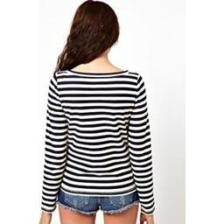
\includegraphics[width=3cm] {../thesis/images/adv/target}};
\node [above=of target, yshift=-1cm, color1, font=\small] {Target};

\node [rectangle, right=1cm of target, inner sep=0.5pt,color2, draw, thick] (original) {
\includegraphics[width=3cm] {../thesis/images/adv/original}};
\node [above=of original, yshift=-1cm, color2, font=\small] {Original};

\node [right=0.25cm of original, inner sep=0.5pt, color4, font=\small] (plus) {$+$};

\node [rectangle, right=0.25cm of plus, inner sep=0.5pt, color4, draw, thick] (pertubation) {
\includegraphics[width=3cm] {../thesis/images/adv/normal-24-epochs/pgd/0.03/pertubation}};
\node [above=of pertubation, yshift=-1cm, color4, font=\small] {Pertubation};

\node [right=0.25cm of pertubation, inner sep=0.5pt, color3, font=\small] (equal) {$=$};

\node [rectangle, right=0.25cm of equal, inner sep=0.5pt, color3, draw, thick] (attack) {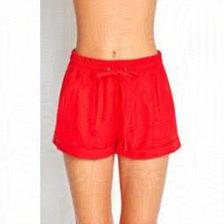
\includegraphics[width=3cm] {../thesis/images/adv/normal-24-epochs/pgd/0.03/attack}};
\node [above=of attack, yshift=-1cm, color3, font=\small] {Adversarial};

\end{tikzpicture}